\subsubsection{\stid{4.14} VeloC: Very Low Overhead Checkpointing System}

\paragraph{Overview.}
The VeloC-SZ project aims to provide VeloC, a high-performance,
scalable checkpoint/restart framework that leverages multi-level
checkpointing (the combination of several resilience strategies and
heterogeneous storage) to ensure that ECP applications run to
completion with minimal performance overhead. It delivers a
production-ready solution that increases development productivity by
reducing the complexity of having to deal with a heterogeneous storage
stack and multiple vendor APIs. VeloC offers a client library that can
be used by the applications to capture local application states, which
are then coordinated and persisted using a resilience engine.  VeloC
runs the resilience engine asynchronously, which overlaps a large part
of the checkpointing with the application runtime, thereby reducing
its overhead. An overview of the architecture of VeloC is depicted
in Figure~\ref{fig:veloc:arch}.

VeloC has been released and shows significant lower checkpointing
overhead for several ECP applications, such as HACC, LatticeQCD,
EXAALT.

\paragraph{Key Challenges.}
VeloC addresses several key challenges:
\vspace{-1em}

\paragraph{\emph{I/O bottlenecks:}} applications typically employ
simple checkpoint-restart mechanisms to survive failures that directly
use a parallel file system. With diminishing I/O bandwidth available
per core, this leads to high checkpointing overhead and is not
sustainable.
\vspace{-1em}

\paragraph{\emph{Deep heterogeneous storage:}} To compensate for
diminishing parallel file system I/O bandwidth per core, the storage
stack is becoming increasingly deeper and heterogeneous: node-local
NVRAM, burst buffers, key-value stores, etc. However, the variety of
vendor APIs and performance characteristics make it difficult for
application developers to take advantage of it.
\vspace{-1em}

\paragraph{\emph{Restart-in-place:}} a majority of failures affect
only a small part of the nodes where the job is running. Therefore,
reusing the surviving nodes to restart from the latest checkpoint
immediately after a failure is more efficient than submitting a new job,
which may wait for a long time in the batch queue.
\vspace{-1em}

\paragraph{\emph{Efficient serialization:}} The critical data structures
of HPC applications that need to be checkpointed are constantly
growing in size and complexity. Manual serialization of such data
structures as contiguous sequences of bytes to be written into
checkpoints is both tedious (leading to loss of productivity) and
inefficient (leading to longer runtime). Therefore, automated
optimized serialization support is needed.

\paragraph{Solution Strategy}

To address these challenges, VeloC adopts the following principles:
\vspace{-1em}

\paragraph{\emph{Multi-level checkpointing:}} is based on the idea
that a majority of failures can be mitigated without involving the
parallel file system: node-local checkpoints can be used to recover
from software bugs, replication/erasure coding can be used to recover
from most combinations of node failures. This reduces the frequency of
checkpointing to the parallel file system and therefore the I/O
bottlenecks.
\vspace{-1em}

\paragraph{\emph{Asynchronous mode:}} once a node-local checkpoint has
been written, applications do not need to wait for replication,
erasure coding or writes to the parallel file system: these can be
applied in the background, while the application continues
running. However, in this case, it is important to minimize
interference with the application execution.
\vspace{-1em}

\paragraph{\emph{Transparent use of heterogeneous storage:}} we
developed several techniques that can leverage a variety of local
storage (in-memory file systems, flash storage) and external storage
(burst buffers, key-value stores, parallel file systems)
options. These techniques select the best available storage options,
tune them with the optimal parameters and leverage any vendor-specific
API if needed to transfer data.
\vspace{-1em}

\paragraph{\emph{Job scheduler integration:}} to implement
restart-in-place, we have developed a series of scripts that interact
with a variety of job schedulers to run jobs with spare nodes,
continue execution on failures, restart on the surviving nodes and
spares using the fastest possible recovery strategy (which ideally
avoids reading checkpoints from the parallel file system). This is
transparent to the users.
\vspace{-1em}

\paragraph{\emph{Declarative API and automated serialization:}} we
offer a simple API that enables users to either manually capture
checkpoints into files or to define memory regions that are
automatically serialized into checkpoint files.
\vspace{-1em}

\paragraph{\emph{Modular design:}} applications link with a client
library that is responsible to manage local checkpoints, while a
separate engine is responsible to employ the rest of the resilience
strategies as plugable modules. This simplifies the implementation
of the asynchronous mode, it enables users the flexibility to choose any
combination of resilience strategies, as well as, to customize their
checkpointing pipeline (e.g., add new post-processing operations such
as analytics or compression).

\paragraph{Recent Progress}

We met and closely collaborated with several ECP application teams in
an effort to address their checkpointing needs. Most of our current
efforts involve the HACC, LatticeQCD, and EXAALT teams. We also
started integrating VELOC into NWChemEX. Based on feedback from
several teams, we extended VELOC to support multiple communication
protocols that reduce dependencies on external libraries (such as
Boost) if desired.  Furthermore, we added preliminary support for
checkpoint aggregation, which reduces the number of checkpoint files
from one per rank to a desired smaller number.

\begin{wrapfigure}{l}{0.47\textwidth}
  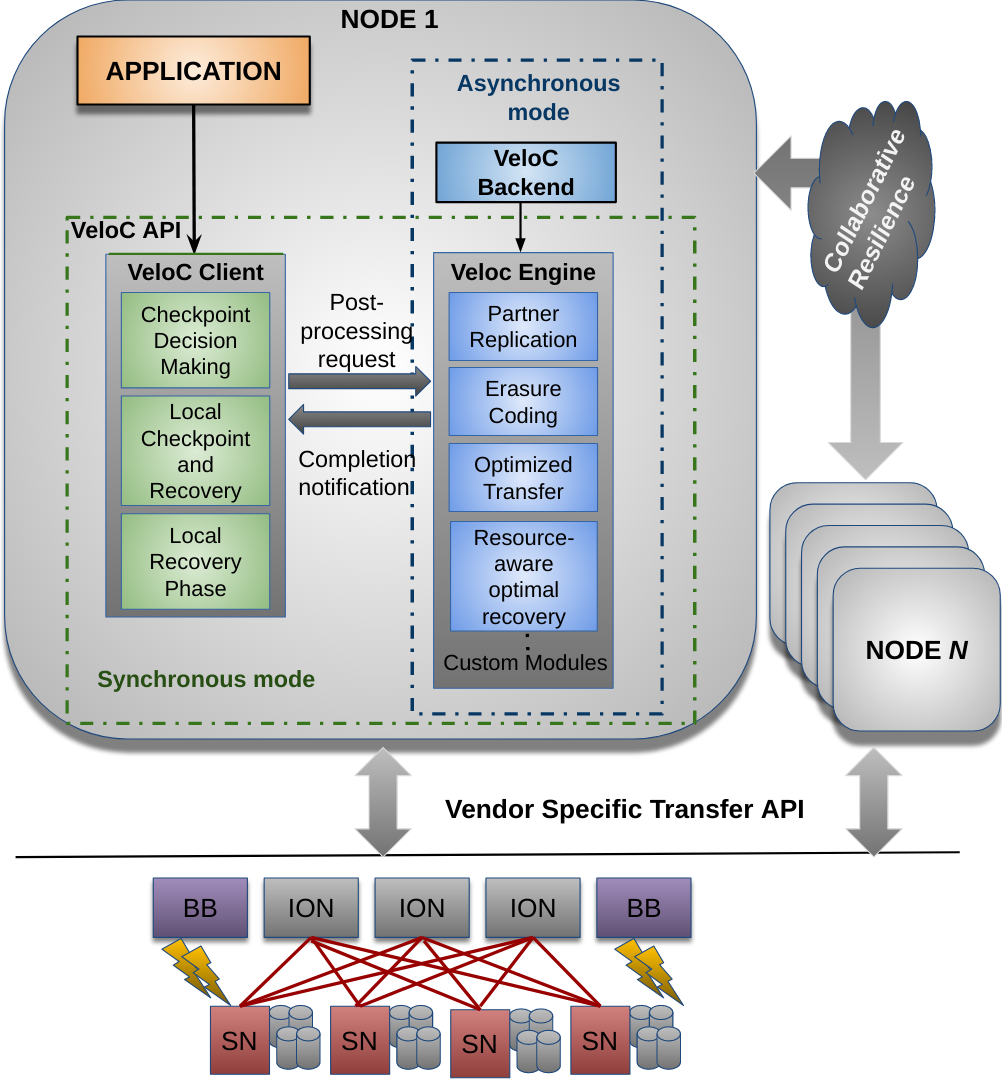
\includegraphics[width=0.4\textwidth]{projects/2.3.4-DataViz/2.3.4.14-VeloC-SZ/veloc-arch}
  \caption{VeloC: Architecture}%
  \label{fig:veloc:arch}%
\end{wrapfigure}

Furthermore, we added several new capabilities. First, we added
support for \emph{serialization} of C++ objects based on the notion
of \emph{lambda serializers}, which register a recipe for
serialization with VELOC that will be used during checkpointing. This
recipe can be individually tuned for each data structure individually
and may potentially mix different serialization libraries within the
same checkpoint. Second, we added support to run the active backend as
an application thread within a leading rank on each compute node. This
approach eliminates the need to deploy an active backend on each
compute node separately.

In addition, we have added several new features that facilitate better
integration with the ECP ecosystem. We extended the series of tests
(originally a minimal set based on Travis and linked with our public
GitHub repository) to include a comprehensive set of combinations of
scenarios, both for VELOC and its subcomponents. Furthermore, we
devised a series of multi-node tests specifically designed for
HPC scenarios running on ECP testbeds. These tests were also integrated
with the continous integration infrastructure maintained by ECP
(which runs in parallel with our Travis integration). Finally, we
are also providing a Spack installation package that is part of the
OpenHPC distribution.

We also started several exploratory directions that resulted in
several research publications. Notably, we explored how to integrate
VELOC with performance-portable asbtractions such as Kokkos. Notably,
we proposed the notion of \emph{resilience portability} based on
checkpointable memory views, which automates the definition of
critical regions (otherwise manually identified by
users)~\cite{PortResEuroPar21}. This research effort continues with
additional support for incremental checkpointing based on
deduplication techniques applied to the memory views. Furthermore, we
proposed several checkpoint aggregation techniques specifically
designed for the asynchronous mode of operation that allows the
application to continue running. In this context, we have explored a
strategy based on parallel POSIX writes to disjoint offsets in the
same file, as well as a strategy based on MPI-IO. A publication that
summarizes our findings is under preparation.

\paragraph{Next Steps}
We are working towards several goals: (1) more advanced checkpoint
aggregation techniques; (2) support for key-value stores as an
alternative to parallel file systems, notably DAOS; (3) continue
hardening the integration with existing ECP applications and automated
testing infrastructure.  In parallel, we will continue to collaborate
with the ECP application teams to address new requirements should they
arise.
